% ==============================================================================
% Section 1.8: Case Study — Pion
% ==============================================================================

\section{Case Study: Pion Decay}
\label{sec:case_pion}

\subsection{\texorpdfstring{Pion Decay: The Hadron$\to$Lepton Bridge}{Pion Decay: The Hadron to Lepton Bridge}}

% --- AT-A-GLANCE BOX (KB-CANON-002) ---
\begin{edcAtAGlance}{Pion Decay}
  \edcBaseline{
    Decay: $\pi^+ \to \mu^+ + \nu_\mu$ (99.988\%) dominant channel\\
    Suppressed: $\pi^+ \to e^+ + \nu_e$ (BR $\approx 1.23 \times 10^{-4}$)\\
    Lifetime: $\tau_\pi \approx 2.60 \times 10^{-8}$ s\\
    Helicity suppression: $(m_e/m_\mu)^2$ scaling well-established
  }
  \edcEDCView{
    Pion = composite junction-pair (distinct from single-mode leptons)\\
    Annihilates and releases energy through brane interface\\
    Chiral projection $\mathcal{P}_{\mathrm{chir}}$ produces helicity suppression\\
    Tests whether boundary conditions can produce lepton-mass sensitivity
  }
  \edcKeyInsight{
    The pion bridges hadrons and leptons: a composite (junction-pair) object
    releasing into pure leptonic outputs. If the same $\mathcal{P}_{\mathrm{frozen}}$
    works here, the interface mechanism transcends the lepton/hadron divide.
  }
  \edcFalsifiable{
    \textbullet\ If BC interpretation cannot accommodate helicity suppression qualitatively\\
    \textbullet\ If composite ontology contradicts lepton single-mode ontology\\
    \textbullet\ If $\pi^0 \to \gamma\gamma$ requires qualitatively different framework
  }
\end{edcAtAGlance}

\medskip

% ==============================================================================
% MOTIVATION
% ==============================================================================

\subsubsection{Motivation: First Hadron$\to$Lepton Test}

The pion is the first place where the EDC weak narrative must confront compositeness.
A pion is not a fundamental lepton-like excitation; it is a composite configuration.
Therefore the goal here is \emph{not} to ``derive'' $m_\pi$ or fit lifetimes, but to define a consistent
ontology and to show how the brane-interface projection can remain compatible with the
observed helicity suppression structure.

\begin{tcolorbox}[edcCornerstone, title=\textbf{Cornerstone: First Hadron$\to$Lepton Test}]
Companions M and T established that the absorption$\to$dissipation$\to$release
pipeline works for \emph{brane-dominant leptonic} decays ($\mu \to e\nu\bar\nu$,
$\tau \to \ell\nu\bar\nu$). The charged pion $\pi^+$ provides the first test
in the \emph{hadronic sector}: a composite object decaying into leptons.
\end{tcolorbox}

\paragraph{Strategic position.}
The pion tests three aspects of the EDC framework:
\begin{enumerate}[label=(\roman*), nosep]
\emergencystretch=2em
    \item \textbf{Ontology test:} Is the pion a different class of 5D object
          than leptons? (Answer: yes---composite vs.\ fundamental.)
    \item \textbf{Pipeline generality:} Does the three-stage pipeline
          (absorption\,$\to$\,dissipation\,$\to$\,release) apply to
          hadron\,$\to$\,lepton transitions?
    \item \textbf{Selection rule test:} Does $\mathcal{P}_{\mathrm{frozen}}$
          account for the $\mu$-dominance over $e$?
\end{enumerate}

\paragraph{Scope and epistemic status.}
This case study is a consistency/ontology paper, not a mass or
lifetime derivation. We test whether the EDC pipeline \emph{accommodates}
pion$\to$lepton transitions without introducing new mechanisms—we do
\textbf{not} claim to derive $m_\pi$, $\tau_\pi$, or the $m_\ell^2$
helicity suppression factor from first principles.

% ==============================================================================
% EPISTEMIC STATUS TABLE
% ==============================================================================

\begin{table}[htbp]
\centering
\caption{Epistemic status of claims in the pion case study}
\label{tab:pion-epistemic-status}
\begin{tabular}{lll}
\toprule
\textbf{Claim} & \textbf{Tag} & \textbf{Status} \\
\midrule
\multicolumn{3}{l}{\textit{Baseline facts (external):}} \\
Helicity suppression $\Gamma \propto m_\ell^2$ & \tagBL{} & SM/PDG \\
$\mu$-channel dominance ($99.99\%$) & \tagBL{} & PDG 2024 \\
Radiative channels exist & \tagBL{} & PDG 2024 \\
$m_\pi$, $\tau_\pi$ values & \tagBL{} & PDG 2024 \\
\midrule
\multicolumn{3}{l}{\textit{EDC postulates:}} \\
Pion = brane-dominant composite & \tagP{} & This paper \\
Absorption$\to$Dissipation$\to$Release applies & \tagP{} & Framework \\
$\mathcal{P}_{\mathrm{chir}}$ qualitatively consistent & \tagP{} & Hypothesis \\
\midrule
\multicolumn{3}{l}{\textit{Open problems:}} \\
Derive $m_\ell^2$ from BC & (open) & Not attempted (OPR-14) \\
Derive $m_\pi$, $\tau_\pi$ & (open) & Not attempted (OPR-16) \\
Junction-pair micro-ontology & (open) & Candidate only (OPR-15) \\
\bottomrule
\end{tabular}
\end{table}

This case study addresses \emph{leptonic} pion decays only. Hadronic modes
(e.g., $\pi^0 \to \gamma\gamma$) require photon ontology and are deferred
to future work (open).

% ==============================================================================
% PION ONTOLOGY
% ==============================================================================

\subsubsection{Pion Ontology: Brane-Dominant Composite Excitation}

\begin{edcPostulateBox}{Pion Ontology}{[P]}
The charged pion $\pi^+$ is a \textbf{brane-dominant composite excitation}
in the hadronic sector. It is localized primarily on the brane layer,
not in the bulk, and consists of a bound configuration of sub-structures
(quarks in the Standard Model picture; localized defects/modes in the EDC
picture).
\end{edcPostulateBox}

\textbf{Physical narration:}
\begin{enumerate}[nosep]
    \item \textbf{5D cause:} A composite bound state forms on the brane layer through
          localization of two correlated defect-modes.
    \item \textbf{Brane response:} The brane supports this metastable configuration
          with a characteristic energy scale $m_\pi c^2 \approx 140$~MeV \tagBL{}.
    \item \textbf{3D output:} Observers detect a spin-0 meson with definite mass and
          charge.
\end{enumerate}

This is distinct from:
\begin{itemize}[nosep]
  \item Leptons ($e$, $\mu$, $\tau$): single brane defects (brane-dominant fundamental)
  \item Neutron: bulk-core junction with proton anchor endpoint
\end{itemize}

% ==============================================================================
% JUNCTION-PAIR MICRO-ONTOLOGY
% ==============================================================================

\subsubsection{Candidate Micro-Ontology: Junction-Pair}

\begin{tcolorbox}[edcConcept, title=\textbf{Junction-Pair Candidate}]
One candidate micro-ontology is a \textbf{defect--antidefect bound state}
(``junction-pair'') on the brane layer \tagP{}. In this picture:
\begin{itemize}[nosep]
    \item The $u$ and $\bar{d}$ quarks correspond to localized junction
          defects of opposite ``charge'' (in the topological sense).
    \item Confinement arises from the brane-layer potential that binds
          the junction-pair at characteristic separation $\sim 1$~fm.
\end{itemize}

\textbf{Key open questions} (open):
\begin{enumerate}[nosep]
    \item Is the binding bulk-facing or observer-facing?
    \item How does color confinement map to 5D topology?
    \item Why $m_\pi \approx 140$~MeV and not another value?
\end{enumerate}
\end{tcolorbox}

% ==============================================================================
% OBSERVATIONAL BASELINES
% ==============================================================================

\subsubsection{Observational Baselines}

\begin{table}[htbp]
\centering
\caption{Charged pion properties (PDG 2024) \tagBL{}}
\label{tab:pion-baselines}
\begin{tabular}{lll}
\toprule
\textbf{Quantity} & \textbf{Value} & \textbf{Tag} \\
\midrule
Mass $m_{\pi^+}$ & $139.570\,39(18)$~MeV/$c^2$ & \tagBL{} \\
Lifetime $\tau_{\pi^+}$ & $2.6033(5) \times 10^{-8}$~s & \tagBL{} \\
BR($\pi^+ \to \mu^+\nu_\mu$) & $99.98770(4)\%$ & \tagBL{} \\
BR($\pi^+ \to e^+\nu_e$) & $1.230(4) \times 10^{-4}$ & \tagBL{} \\
\bottomrule
\end{tabular}
\end{table}

The ratio BR($\mu$)/BR($e$) $\approx 8100$ is the \emph{helicity
suppression} phenomenon \tagBL{}.

\textbf{Other decay channels:}
Additional channels exist at sub-dominant levels \tagBL{}: radiative decays
$\pi^+ \to \ell^+\nu_\ell\gamma$ (BR $\sim 10^{-4}$--$10^{-8}$), and
rare/forbidden modes tested by precision experiments. This case study
focuses on the dominant leptonic channels; radiative modes require
photon ontology and are flagged (open).

% ==============================================================================
% PIPELINE FOR PION DECAY
% ==============================================================================

\subsubsection{Pipeline for Pion Decay}

The pion decay follows the same three-stage pipeline as leptonic decays:

\begin{tcolorbox}[edcPPN, title=\textbf{Physical Process Narrative: Pion Leptonic Decay}]
\begin{enumerate}[nosep]
    \item[\textbf{(i)}] \textbf{Absorption:} The composite pion excitation becomes
          unstable and its energy is absorbed into the brane-layer
          dissipation channel.
    \item[\textbf{(ii)}] \textbf{Dissipation:} Energy redistributes through brane
          modes, subject to conservation laws (charge, lepton number,
          spin, energy-momentum).
    \item[\textbf{(iii)}] \textbf{Release:} The frozen projection $\mathcal{P}_{\mathrm{frozen}}$
          selects allowed output configurations; observers detect
          $\ell^+ + \nu_\ell$.
\end{enumerate}
\end{tcolorbox}

Mechanistically, the pion must first be represented as a composite brane/boundary excitation,
then released via $\mathcal{P}_{\mathrm{frozen}}$ into lepton + neutrino outputs,
subject to kinematic allowance and chirality selection:
\begin{equation}
\Psi_\pi \;\Rightarrow\; E_{\mathrm{brane/boundary}} \;\Rightarrow\; \mathcal{P}_{\mathrm{frozen}}
\;\Rightarrow\; \ell^+ + \nu_\ell + \text{(recoil/soft)}.
\label{eq:pion_pipeline}
\end{equation}

\paragraph{Key difference from leptonic decays.}
In muon and tau decay, the initial state is a \emph{fundamental} brane-dominant
mode. In pion decay, the initial state is a \emph{composite} brane-dominant
excitation. The pipeline structure is the same; the input ontology differs.

% ==============================================================================
% PROCESS DIAGRAM
% ==============================================================================

\subsubsection{Process Diagram: Pion Decay}

\begin{figure}[htbp]
\centering
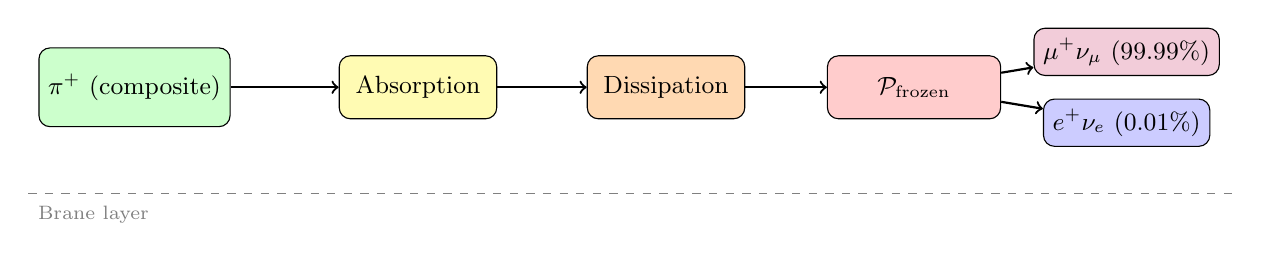
\begin{tikzpicture}[scale=0.9, every node/.style={font=\small}]
    % Pion initial state (composite)
    \node[draw, rounded corners, fill=green!20, minimum width=2cm, minimum height=1cm]
        (pion) at (0,0) {$\pi^+$ (composite)};

    % Absorption stage
    \node[draw, rounded corners, fill=yellow!30, minimum width=2cm, minimum height=0.8cm]
        (abs) at (4,0) {Absorption};

    % Dissipation stage
    \node[draw, rounded corners, fill=orange!30, minimum width=2cm, minimum height=0.8cm]
        (diss) at (7.5,0) {Dissipation};

    % Projection operator
    \node[draw, rounded corners, fill=red!20, minimum width=2.2cm, minimum height=0.8cm]
        (proj) at (11,0) {$\mathcal{P}_{\mathrm{frozen}}$};

    % Output channels
    \node[draw, rounded corners, fill=purple!20, minimum width=1.8cm, minimum height=0.6cm]
        (mu) at (14,0.5) {$\mu^+\nu_\mu$ (99.99\%)};
    \node[draw, rounded corners, fill=blue!20, minimum width=1.8cm, minimum height=0.6cm]
        (e) at (14,-0.5) {$e^+\nu_e$ (0.01\%)};

    % Arrows
    \draw[->, thick] (pion) -- (abs);
    \draw[->, thick] (abs) -- (diss);
    \draw[->, thick] (diss) -- (proj);
    \draw[->, thick] (proj) -- (mu);
    \draw[->, thick] (proj) -- (e);

    % Brane layer indication
    \draw[dashed, gray] (-1.5,-1.5) -- (15.5,-1.5);
    \node[gray, anchor=west, font=\scriptsize] at (-1.5,-1.8) {Brane layer};
\end{tikzpicture}
\caption{Energy flow in charged pion leptonic decay. The pipeline is
identical to muon/tau decay, with the pion as initial composite state.
The projection operator $\mathcal{P}_{\mathrm{frozen}}$ strongly favors
the $\mu$-channel \tagBL{}.}
\label{fig:pion_pipeline}
\end{figure}

% ==============================================================================
% ENERGY BOOKKEEPING
% ==============================================================================

\subsubsection{Energy Bookkeeping Ledger}

\begin{table}[htbp]
\centering
\caption{Energy ledger for $\pi^+ \to \ell^+\nu_\ell$ (qualitative, no fitted values)}
\label{tab:pion-energy-ledger}
\begin{tabular}{lll}
\toprule
\textbf{Stage} & \textbf{Energy Location} & \textbf{Tag} \\
\midrule
Initial & Composite binding (brane-layer) & \tagP{} \\
Absorption & Transferred to dissipation modes & \tagP{} \\
Dissipation & Redistributed among brane modes & \tagP{} \\
Release & $\ell^+$ kinetic + $\nu_\ell$ kinetic & \tagDc{} \\
\midrule
Bulk leakage & Suppressed (brane-dominant) & \tagP{} \\
\bottomrule
\end{tabular}
\end{table}

\textbf{Ledger conservation:} Total energy $m_\pi c^2$ is conserved
through all stages. The ``suppressed bulk leakage'' assumption \tagP{} ensures
that energy remains on the brane layer until release through allowed channels.

% ==============================================================================
% HELICITY SUPPRESSION
% ==============================================================================

\subsubsection{Helicity Suppression: Baseline vs.\ EDC Interpretation}

\paragraph{Standard Model scaling \tagBL{}.}
Experimentally, the charged pion decay rates satisfy a strong lepton-mass dependence:
\begin{equation}
\Gamma(\pi^+ \to \ell^+\nu_\ell) \propto m_\ell^2 \left(1 - \frac{m_\ell^2}{m_\pi^2}\right)^2
\label{eq:sm-helicity-scaling}
\end{equation}
This gives BR($\mu$)/BR($e$) $\approx (m_\mu/m_e)^2 \times (\text{phase space})
\approx 8100$, matching observation \tagBL{}.

The physical origin in SM: the pion has spin-0, so the $\ell^+\nu_\ell$ pair
must have total spin-0. Angular momentum conservation forces a helicity
mismatch for the charged lepton. Lighter leptons have smaller ``wrong helicity''
amplitude, suppressed by $m_\ell$.

\paragraph{EDC projection mechanism \tagP{}.}

\begin{edcPostulateBox}{Projection Mechanism for Helicity Suppression (open)}{[P]}
In the EDC framework, the frozen projection operator
\begin{equation}
\mathcal{P}_{\mathrm{frozen}} = \mathcal{P}_{\mathrm{energy}} \circ
\mathcal{P}_{\mathrm{mode}} \circ \mathcal{P}_{\mathrm{chir}}
\label{eq:pion-projection-stack}
\end{equation}
includes a chiral filter $\mathcal{P}_{\mathrm{chir}}$ that acts on
both the decaying composite and the outgoing lepton.

The filter preferentially allows channels where the outgoing charged
lepton can support the required chirality configuration on the brane
boundary. The mismatch scales with the lepton mass parameter that
characterizes chirality mixing.
\end{edcPostulateBox}

\textbf{Physical narration:}
\begin{enumerate}[nosep]
    \item \textbf{5D cause:} The brane boundary conditions impose chirality
          constraints on allowed final states.
    \item \textbf{Brane response:} The chiral filter $\mathcal{P}_{\mathrm{chir}}$
          projects out configurations with insufficient chirality overlap.
    \item \textbf{3D output:} Observers see $\mu$-channel dominance because the
          heavier muon has larger chirality overlap with the pion's release
          configuration.
\end{enumerate}

\paragraph{Derivation status (open).}
Deriving the $m_\ell^2$ scaling from explicit boundary-condition
computation remains \textbf{open}. Required steps:
\begin{enumerate}[nosep]
    \item Specify the pion's brane-layer wavefunction (composite structure).
    \item Compute the overlap integral with outgoing lepton modes.
    \item Show that the overlap scales as $m_\ell$ (giving $m_\ell^2$ in rate).
\end{enumerate}
Until this is done, we treat the $m_\ell^2$ scaling as \tagBL{} and the
projection mechanism as \tagP{}.

\begin{tcolorbox}[edcWarning, title=\textbf{Guardrail: No $m_\ell^2$ Derivation}]
\textbf{This case study does NOT derive the $m_\ell^2$ helicity suppression
factor.} We accept it as a baseline fact \tagBL{} and show that the EDC
chiral-filter hypothesis is \emph{qualitatively consistent} with the
observed $\mu$-dominance. The explicit boundary-condition computation
that would produce $m_\ell^2$ is flagged (open).
\end{tcolorbox}

% ==============================================================================
% METASTABILITY MECHANISM
% ==============================================================================

\subsubsection{Pion Metastability}

Why does the pion exist as a metastable object with $\tau_\pi \approx 26$~ns?

\begin{edcPostulateBox}{Metastability Mechanism (open)}{[P]}
The pion is metastable because:
\begin{enumerate}[nosep]
    \item \textbf{Brane localization:} The junction-pair (or equivalent
          composite) is confined to the brane layer by a localization
          potential (spectral gap).
    \item \textbf{Suppressed release:} The only allowed release channels
          ($\ell^+\nu_\ell$) require ``unwinding'' the composite through
          the frozen projection, which is kinematically constrained.
    \item \textbf{No bulk escape:} Direct bulk dissipation is suppressed
          for brane-dominant composites (same as for leptons).
\end{enumerate}
\end{edcPostulateBox}

\textbf{Physical narration:}
\begin{enumerate}[nosep]
    \item \textbf{5D cause:} The brane layer has a spectral gap that traps
          composite excitations.
    \item \textbf{Brane response:} The composite remains localized until it can
          release through allowed leptonic channels.
    \item \textbf{3D output:} Observers detect a particle with finite lifetime
          $\tau_\pi \approx 26$~ns \tagBL{}.
\end{enumerate}

\textbf{No mass derivation:}
We do \textbf{not} attempt to derive $m_\pi = 140$~MeV from first
principles. This requires a complete theory of quark/defect binding
in the 5D framework, which is (open).

% ==============================================================================
% ALLOWED OUTPUT SETS
% ==============================================================================

\subsubsection{Allowed Output Sets}

\begin{edcDefinitionBox}{Allowed Outputs for $\pi^+$ Decay}{[Dc]}
The allowed output set for $\pi^+$ leptonic decay is:
\begin{equation}
\mathcal{A}_{\pi^+} = \{(\mu^+, \nu_\mu), (e^+, \nu_e)\}
\label{eq:pion_allowed_outputs}
\end{equation}
Both channels satisfy:
\begin{itemize}[nosep]
    \item Charge conservation: $+1 \to +1 + 0$
    \item Lepton number: $0 \to (-1)_{\ell^+} + (+1)_{\nu_\ell} = 0$
    \item Energy-momentum: $m_\pi c^2 > m_\ell c^2 + 0$ (kinematically allowed)
    \item Spin: $0 \to \frac{1}{2} + \frac{1}{2}$ (total spin-0 possible)
\end{itemize}
\end{edcDefinitionBox}

% ==============================================================================
% CHANNELS TABLE
% ==============================================================================

\subsubsection{Leptonic and Forbidden Channels}

\begin{table}[htbp]
\centering
\caption{Pion leptonic channels: experimental vs.\ EDC framing}
\label{tab:pion-channels}
\begin{tabular}{llll}
\toprule
\textbf{Channel} & \textbf{BR (Exp)} & \textbf{EDC Status} & \textbf{Tag} \\
\midrule
$\pi^+ \to \mu^+\nu_\mu$ & $99.99\%$ & Allowed; projection-favored & \tagDc{} \\
$\pi^+ \to e^+\nu_e$ & $0.01\%$ & Allowed; projection-suppressed & \tagDc{} \\
$\pi^+ \to \gamma + X$ & Various & Requires photon ontology & (open) \\
\bottomrule
\end{tabular}
\end{table}

% ==============================================================================
% CHIRAL FILTER UNIVERSAL HYPOTHESIS
% ==============================================================================

\subsubsection{Chiral Filter: Universal Hypothesis}

The chiral projection $\mathcal{P}_{\mathrm{chir}}$ is hypothesized to
arise from brane boundary conditions \tagP{}. For pion decay, the
relevant constraint is:

\begin{quote}
\emph{The spin-0 pion must release into a lepton-neutrino pair with
total spin-0. The chiral filter preferentially selects configurations
where the charged lepton's helicity mismatch is minimized—favoring
heavier leptons.}
\end{quote}

This is qualitatively consistent with the SM helicity suppression,
but the explicit boundary-condition derivation is (open).

\begin{tcolorbox}[mechanism, title={Universal Chiral Filter Hypothesis}]
\textbf{Hypothesis} \tagP{}\textbf{:} We hypothesize that the same
$\mathcal{P}_{\mathrm{chir}}$ acts in all weak decays (muon, tau, pion, neutron).
If true, this would unify the selection-rule structure across the EDC weak program.
\end{tcolorbox}

% ==============================================================================
% LEDGER CLOSURE
% ==============================================================================

\subsubsection{Ledger Closure}

\begin{edcLedgerBox}{Pion bookkeeping}{[Dc]}
\begin{equation}
m_\pi c^2 = E_{\ell^+} + E_{\nu_\ell} + E_{\mathrm{soft}} + E_{\mathrm{recoil}},
\label{eq:pion_ledger}
\end{equation}
where the lepton and neutrino carry the bulk of the released energy, with
small soft/recoil corrections.
\end{edcLedgerBox}

% ==============================================================================
% WHY PION MATTERS
% ==============================================================================

\subsubsection{Why the Pion Case Matters}

{%
\emergencystretch=3em
The pion is the \emph{lightest hadron} and the first composite object
to undergo the hadron\,$\to$\,lepton transition in the EDC weak program.
Its successful accommodation by the absorption\,$\to$\,dissipation\,$\to$\,release
pipeline demonstrates that:\par
}%
\begin{enumerate}[nosep]
    \item The pipeline is \textbf{not restricted to fundamental particles}—it
          generalizes to composite brane excitations.
    \item The \textbf{ontological distinction} (fundamental vs.\ composite,
          brane-dominant vs.\ bulk-core) is physically meaningful within EDC.
    \item The chiral filter hypothesis gains support from a \textbf{third
          particle sector} (hadrons), beyond the lepton-only tests (M, T).
\end{enumerate}

% ==============================================================================
% FALSIFIABILITY HOOKS
% ==============================================================================

\subsubsection{Falsifiability Hooks}

\begin{tcolorbox}[falsifiability, title=\textbf{Falsifiability: What Would Refute This Framing?}]
\begin{enumerate}[nosep]
    \item \textbf{Ontology:} If the pion's 5D structure is shown to be
          bulk-dominant (not brane-dominant), the ontology postulate \tagP{} fails.
    \item \textbf{Pipeline:} If pion decay requires a fundamentally
          different mechanism than absorption$\to$dissipation$\to$release,
          the framework generalization fails.
    \item \textbf{Selection rules:} If allowed channels violate the
          $\mathcal{A}_{\pi^+}$ set (e.g., $\pi^+ \to \gamma\gamma$
          becomes dominant over leptonic), the selection rules fail.
    \item \textbf{Helicity suppression:} If future EDC derivation of
          $\mathcal{P}_{\mathrm{chir}}$ predicts $e$-dominance over $\mu$,
          the chiral-filter mechanism fails.
    \item \textbf{Ledger consistency:} If energy bookkeeping cannot close
          (i.e., $m_\pi c^2 \neq E_{\ell} + E_\nu$ within experimental
          precision), the ledger conservation assumption fails.
    \item \textbf{Universality:} If the chiral filter must be different
          for pions than for leptons (M, T), the universal hypothesis fails.
\end{enumerate}
\end{tcolorbox}

% ==============================================================================
% OPEN PROBLEMS
% ==============================================================================

\subsubsection{Open Problems}

\begin{enumerate}[nosep]
    \item \textbf{Derive $m_\pi$ from 5D binding} (open): What determines
          $m_\pi \approx 140$~MeV?
    \item \textbf{Derive $\tau_\pi$ from first principles} (open): Why
          $\tau_\pi \approx 26$~ns?
    \item \textbf{Derive $m_\ell^2$ scaling from BC} (open): Show that
          boundary conditions produce the helicity suppression factor.
    \item \textbf{Junction-pair micro-ontology} (open): Is the defect--antidefect
          picture correct? How does color confinement map to 5D?
    \item \textbf{Neutral pion $\pi^0 \to \gamma\gamma$} (open): Requires
          photon ontology.
    \item \textbf{Pion-nucleon interactions} (open): How do pions couple
          to bulk-core junctions (neutrons/protons)?
\end{enumerate}

% ==============================================================================
% POSITION IN EDC WEAK PROGRAM
% ==============================================================================

\subsubsection{Position in the EDC Weak Program}

\begin{table}[htbp]
\centering
\caption{EDC Weak Program: ontology comparison}
\label{tab:pion-position}
\begin{tabular}{llll}
\toprule
\textbf{Companion} & \textbf{Particle} & \textbf{Ontology} & \textbf{Initial Sector} \\
\midrule
N & Neutron & Bulk-core junction & Hadronic (baryon) \\
M & Muon & Brane-dominant (fundamental) & Leptonic \\
T & Tau & Brane-dominant (higher mode) & Leptonic \\
\textbf{P} & \textbf{Pion} & \textbf{Brane-dominant (composite)} & \textbf{Hadronic (meson)} \\
\bottomrule
\end{tabular}
\end{table}

% ==============================================================================
% CANONICAL GLOSSARY
% ==============================================================================

\subsubsection{Canonical Glossary for Pion Decay}

\begin{tcolorbox}[edcCanonical, title=\textbf{Canonical Terms: Pion Decay Pipeline}]
\begin{description}[nosep, leftmargin=!, labelwidth=4cm]
\item[Composite excitation] Bound state of multiple defects/modes on brane
\item[Junction-pair] Candidate micro-ontology: defect--antidefect pair
\item[Helicity suppression] $\Gamma \propto m_\ell^2$ scaling (baseline fact)
\item[$\mathcal{A}_{\pi^+}$] Allowed output set: $\{(\mu^+,\nu_\mu), (e^+,\nu_e)\}$
\item[Spectral gap] Brane-layer potential that traps composite excitations
\item[Metastability] Finite lifetime from suppressed release channels
\item[Hadron$\to$lepton bridge] Pion as first composite-to-lepton test
\end{description}
\end{tcolorbox}

% ==============================================================================
% STOPLIGHT VERDICT (2026-01-29)
% ==============================================================================
\subsubsection{Stoplight Verdict}
\label{subsec:pion_stoplight}

\begin{tcolorbox}[colback=yellow!10!white, colframe=orange!60!black,
    title=\textbf{Case Pion: Stoplight Verdict}]

\begin{center}
\begin{tabular}{@{}lll@{}}
\toprule
\textbf{Claim} & \textbf{Status} & \textbf{Tag} \\
\midrule
Composite excitation ontology & \textcolor{YellowOrange}{\textbf{YELLOW}} & \tagP{} \\
Helicity suppression ($\propto m_\ell^2$) & \textcolor{OliveGreen}{\textbf{GREEN}} & \tagBL{}/\tagDc{} \\
Junction-pair micro-ontology & \textcolor{BrickRed}{\textbf{RED}} & \tagP{} (open) \\
$\tau_\pi$ value & \textcolor{BrickRed}{\textbf{RED}} & \tagBL{} (not derived) \\
\bottomrule
\end{tabular}
\end{center}

\textbf{Overall: YELLOW} --- Helicity suppression reproduced; composite structure
not derived from 5D action.

\textbf{Blockers:}
\begin{itemize}[nosep]
\item Composite state derivation from brane topology
\item Junction-pair binding mechanism
\item Quantitative decay rate from mode overlap
\end{itemize}

See \S\ref{sec:gate_registry} for consolidated gate registry.
\end{tcolorbox}


